% !Mode:: "TeX:UTF-8" 



\BiSection{2.25}{Figures}

\fancyhead[R]{本题2.25由QC.Z完成}

		\begin{figure}[H] %H为当前位置,!htb为忽略美学标准,htbp为浮动图形
	\begin{minipage}{\linewidth}
		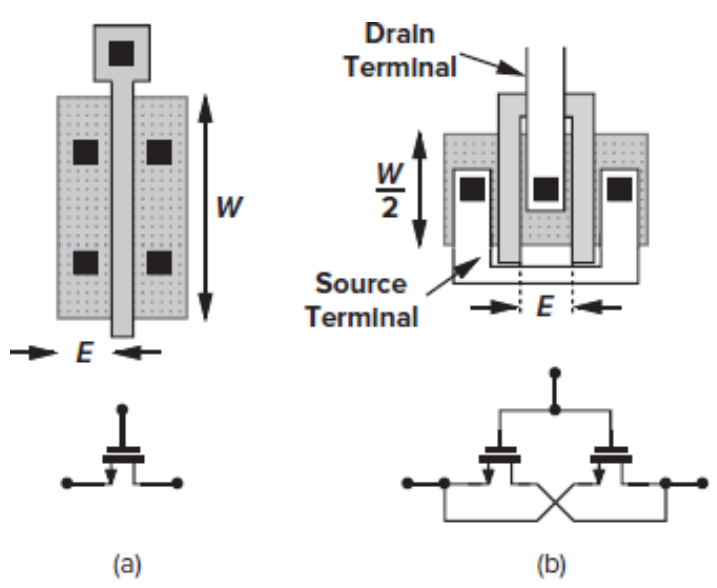
\includegraphics[width=1\linewidth]{2.33-s}
	\end{minipage}
	\caption*{图2.33} %最终文档中希望显示的图片标题
\end{figure}

解:

考虑$L=0.5\mu m$

$V_{DS}=V_{GS}-V_{TH}$

$V_{GS}=V_{DS}+V_{TH}=0.4V+0.7V=1.1V$

$C_{ox}=\frac{\epsilon_{ox}}{T_{ox}}=\frac{3.9 \times 8.854 \times 10^{-12}\frac{F}{m}}{9 \times 10^{-9}m}=3.837 \times 10^{-3}\frac{F}{m^2}$

$I_D=\frac{1}{2}\mu_nC_{ox}\frac{W}{L_{eff}}(V_{GS}-V_{TH})^2=\frac{1}{2}\mu_nC_{ox}\frac{W}{0.5\mu m-2L_D}(V_{GS}-V_{TH})^2$

\begin{figure}[H] %H为当前位置,!htb为忽略美学标准,htbp为浮动图形
	\begin{minipage}{\linewidth}
		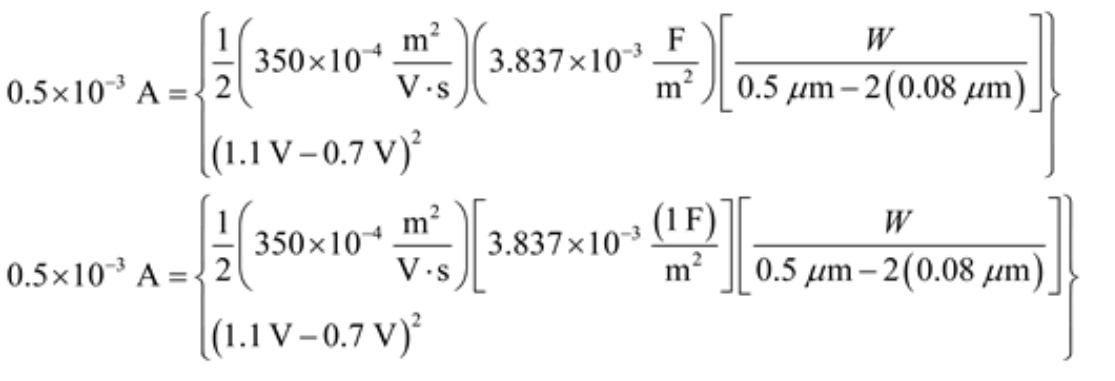
\includegraphics[width=1\linewidth]{2.25-1}
	\end{minipage}
\end{figure}

\begin{figure}[H] %H为当前位置,!htb为忽略美学标准,htbp为浮动图形
	\begin{minipage}{\linewidth}
		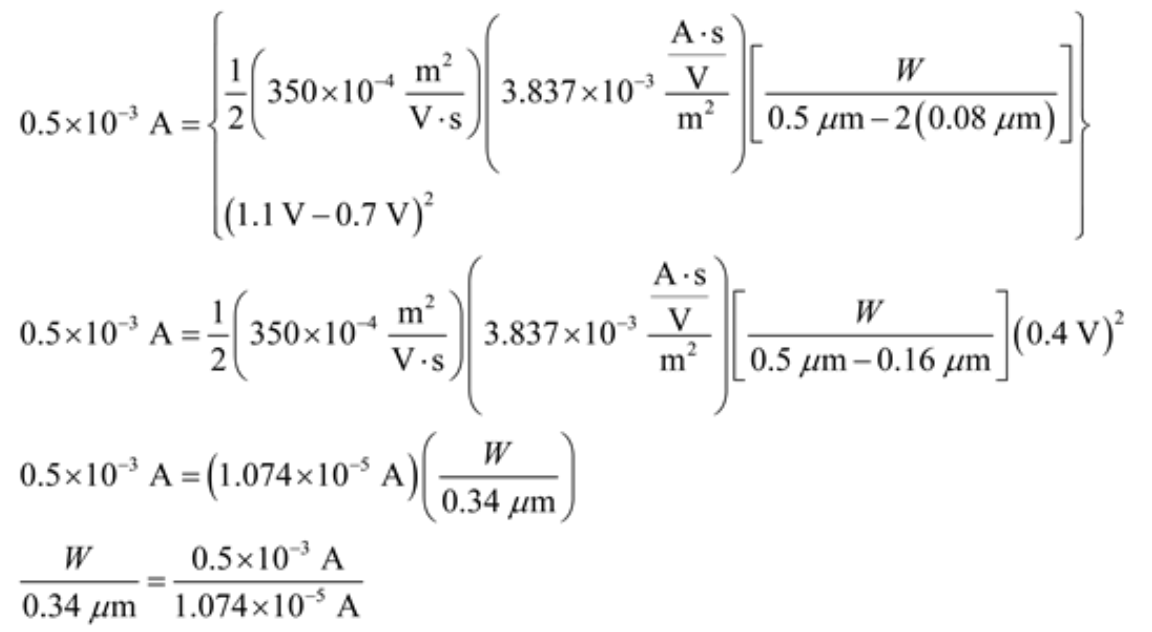
\includegraphics[width=1\linewidth]{2.25-2}
	\end{minipage}
\end{figure}

\begin{figure}[H] %H为当前位置,!htb为忽略美学标准,htbp为浮动图形
	\begin{minipage}{\linewidth}
		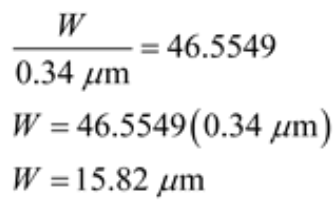
\includegraphics{2.25-3}
	\end{minipage}
\end{figure}

$C_{ov}\cong L_DC_{ox}$

由图2.33,$C_{GS}=\frac{2WLC_{ox}}{3}+WC_{ov}=\frac{2WLC_{ox}}{3}+WL_DC_{ox}$

\begin{figure}[H] %H为当前位置,!htb为忽略美学标准,htbp为浮动图形
	\begin{minipage}{\linewidth}
		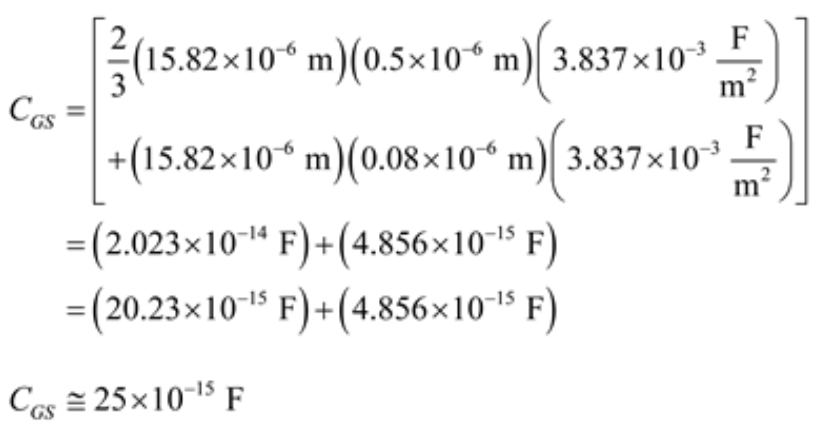
\includegraphics{2.25-4}
	\end{minipage}
\end{figure}

$1f=10^{-15}$

$C_{GS}=25fF$

由图2.33,$C_{GD}=WC_{ov}=WL_DC_{ox}$

\begin{figure}[H] %H为当前位置,!htb为忽略美学标准,htbp为浮动图形
	\begin{minipage}{\linewidth}
		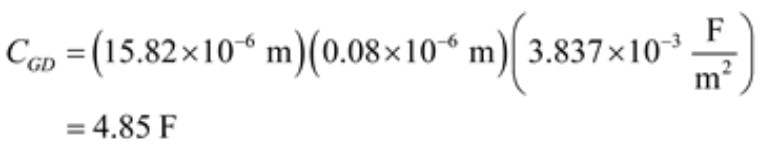
\includegraphics[width=1\linewidth]{2.25-5}
	\end{minipage}
\end{figure}

$C_{DB}=\frac{W}{2}EC_j+2(\frac{W}{2}+E)C_{jsw}$


\begin{figure}[H] %H为当前位置,!htb为忽略美学标准,htbp为浮动图形
	\begin{minipage}{\linewidth}
		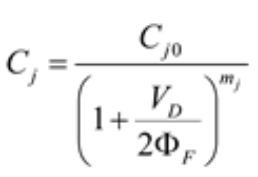
\includegraphics{2.25-6}
	\end{minipage}
\end{figure}

\begin{figure}[H] %H为当前位置,!htb为忽略美学标准,htbp为浮动图形
	\begin{minipage}{\linewidth}
		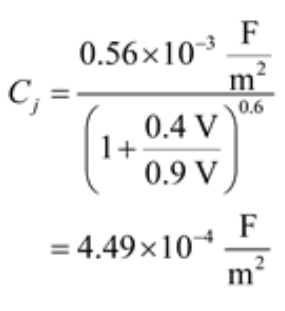
\includegraphics{2.25-7}
	\end{minipage}
\end{figure}

\begin{figure}[H] %H为当前位置,!htb为忽略美学标准,htbp为浮动图形
	\begin{minipage}{\linewidth}
		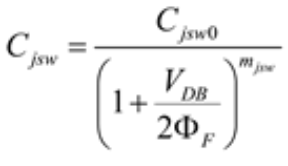
\includegraphics{2.25-8}
	\end{minipage}
\end{figure}

\begin{figure}[H] %H为当前位置,!htb为忽略美学标准,htbp为浮动图形
	\begin{minipage}{\linewidth}
		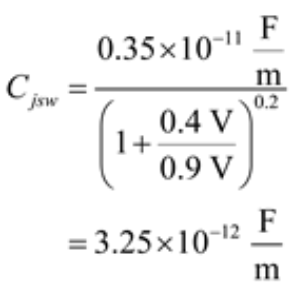
\includegraphics{2.25-9}
	\end{minipage}
\end{figure}

\begin{figure}[H] %H为当前位置,!htb为忽略美学标准,htbp为浮动图形
	\begin{minipage}{\linewidth}
		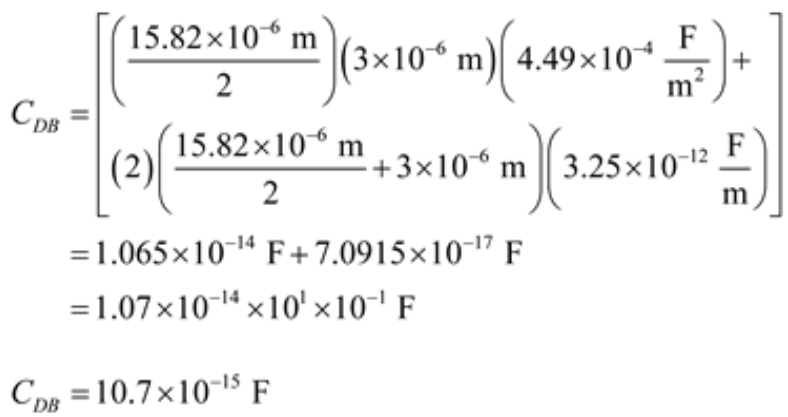
\includegraphics{2.25-10}
	\end{minipage}
\end{figure}














$C_{DB}=10.7fF$